
\documentclass{article}
\usepackage{amsmath}
\usepackage{amssymb}
\usepackage{amsfonts}
\usepackage{graphicx}

\providecommand{\abs}[1]{\left\vert#1\right\vert}
\let\vec\mathbf

\begin{document}

\title{\textbf{GATE IN2023}}
\date{}
\maketitle
\begin{enumerate}
\item In the circuit shown, the initial binary content of shift register A is 1101 and that of shift register B is 1010.The shift registers are positive edge triggered, and the gates have no delay.

When the shift control is high,what will be the binary content of the shift registers A and B after four clock pulses?

		\begin{figure}[!ht]
			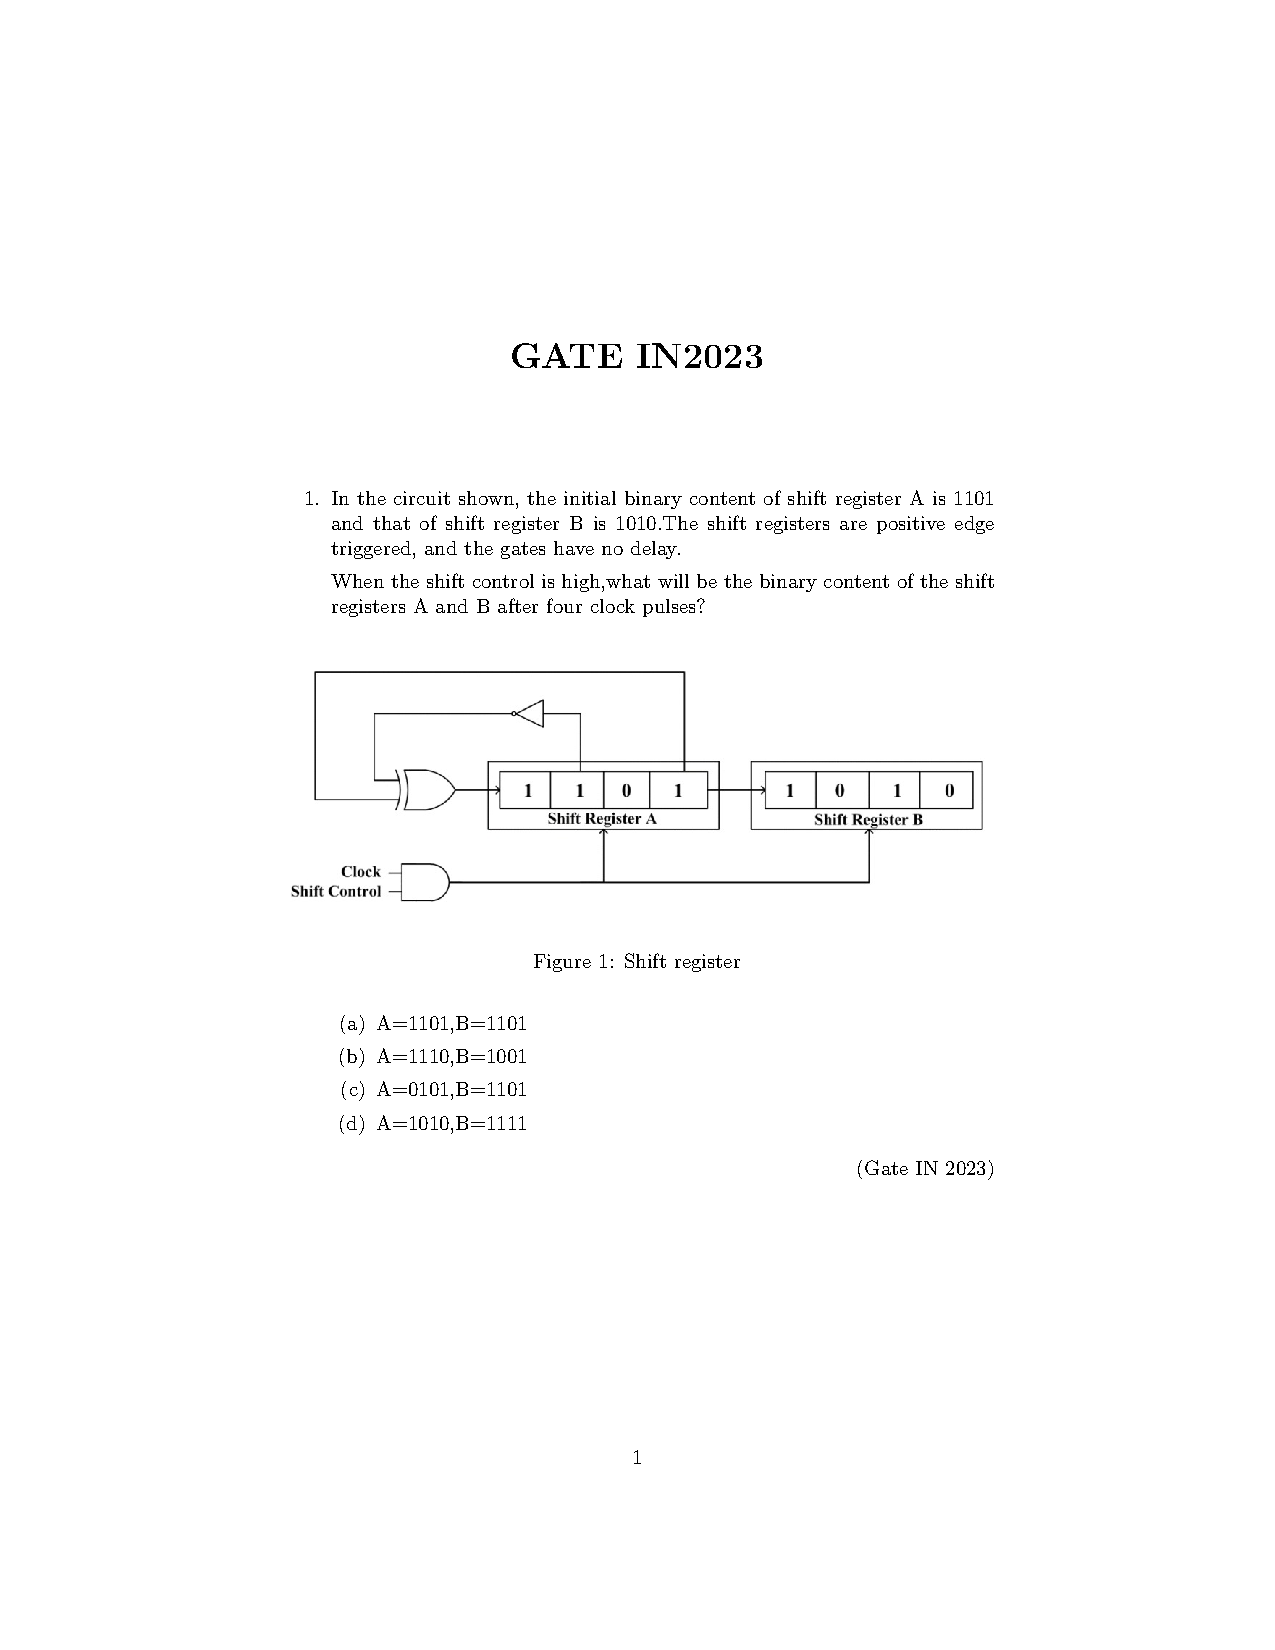
\includegraphics[width=\columnwidth]{figs/gate}
			\caption{Shift register}
			\label{figs:fig1}
		\end{figure}
		\begin{enumerate}
  \item A=1101,B=1101
  \item A=1110,B=1001
  \item A=0101,B=1101
  \item A=1010,B=1111
\end{enumerate}
		\hfill{(Gate IN 2023)}

\end{enumerate}
\end{document}
